\def\resdir{6services}

% ----------------------------------------------------------------------
\section{Services R�seaux}
% ----------------------------------------------------------------------


% ----------------------------------------------------------------------
\subsection{Services}
% ----------------------------------------------------------------------



% ----------------------------------------------------------------------
\begin{frame}{Services R�seaux}

Ensemble des services permettant le fonctionnement des r�seaux locaux
	\begin{itemize}
	\item<+-> Mat�riel et/ou logiciel (\textit{``serveur''})
	\end{itemize}


\begin{itemize}
\item<+-> Attribution des addresses IP et noms de machines
\item<+-> Gestion des
	\begin{itemize}
	\item<+-> Utilisateurs
	\item<+-> Fichiers
	\item<+-> Donn�es
	\item<+-> Impressions	
	\end{itemize}
\item<+-> S�curit�
	\begin{itemize}
	\item<+-> Transversal
	\item<+-> D�di�
	\end{itemize}
\end{itemize}

\end{frame}
% ----------------------------------------------------------------------

% ----------------------------------------------------------------------
\begin{frame}{Services R�seaux : IP}

\begin{block}{Serveur DHCP ; Attribution des addresses IP et noms de machines}
	\begin{itemize}
	\item<+-> \textit{Dynamic Host Configuration Protocol}
	\item<+-> Limite le nombre d'adresses IP
	\item<+-> Facilite la configuration
	\item<+-> Permet l'acc�s aux machines nomades
	\item<+-> Fonctionnement
		\begin{itemize}
		\item<+-> Requ�te \textit{broadcast} TCP/IP \textbf{DHCP DISCOVER}
		\item<+-> R�ponse \textbf{DHCP DISCOVER} contenant
			\begin{itemize}
			\item<+-> Adresse IP + masque de sous-r�seau
			\item<+-> Adresse IP de la passerelle par d�faut
			\item<+-> Adresses IP des serveurs DNS
			\item<+-> Adresses IP des serveurs NBNS (WINS)
			\end{itemize}				
		\end{itemize}		
	\end{itemize}
\end{block}

\end{frame}
% ----------------------------------------------------------------------

% ----------------------------------------------------------------------
\begin{frame}{Gestions - Utilisateurs}

\begin{block}{Annuaires}
	\begin{itemize}
	\item<+-> Notions de groupes et de droits
	\item<+-> Annuaires
		\begin{itemize}
		\item<+-> Active Directory : LDAP + Kerberos
		\item<+-> Contient toutes les informations utilisateurs
		\item<+-> Hi�rarchis�
		\end{itemize}		
	\end{itemize}		
\end{block}

\end{frame}
% ----------------------------------------------------------------------


% ----------------------------------------------------------------------
\begin{frame}{Gestions - Fichiers /donn�es}

\begin{block}<+->{Serveurs de fichiers}
	\begin{itemize}
	\item<+-> Partage des comptes utilisateurs
		\begin{itemize}
		\item<+-> NFS : Network File System
		\end{itemize}
	\item<+-> FTP : File Transfer Protocol
	\item<+-> Samba 
		\begin{itemize}
		\item<+-> Multi-protocoles
		\item<+-> Multi-plateformes
		\end{itemize}
	\end{itemize}
\end{block}

\begin{block}<+->{Serveur de Bases de Donn�es}
	\begin{itemize}
	\item<+-> SGBD (MySQL, PostgreSQL, Oracle\ldots)
	\item<+-> Stockage/sauvegarde
	\item<+-> Des donn�es m�tiers/applicatives
	\end{itemize}
\end{block}


\end{frame}
% ----------------------------------------------------------------------

% ----------------------------------------------------------------------
\begin{frame}{Gestions - Impression}

\begin{block}{Serveurs d'impression}
	\begin{itemize}
	\item<+-> Partage de plusieurs imprimantes
	\item<+-> Entre plusieurs utilisateurs
		\begin{itemize}
		\item<+-> Interfac� � LDAP
		\item<+-> Connection directe (USB) ou r�seau
		\end{itemize}
	\item<+-> Sous linux : CUPS (Common Unix Printing System)
	\end{itemize}
\end{block}

\end{frame}
% ----------------------------------------------------------------------

% ----------------------------------------------------------------------
\begin{frame}{S�curit�}

Transversal et D�di�

\begin{block}{Parefeu / DMZ}
	\begin{itemize}
	\item<+-> Pare-feu : filtrage des communications
	\item<+-> DMZ : DeMilitarized Zone
		\begin{itemize}
		\item<+-> Zone isol�e du reste du r�seau
		\item<+-> Par 1 ou 2 pares-feux
		\end{itemize}
	\item<+-> Sous linux : CUPS (Common Unix Printing System)
	\end{itemize}
\end{block}

\end{frame}
% ----------------------------------------------------------------------


% ----------------------------------------------------------------------
\begin{frame}{S�curit�}

Transversal et D�di�

\begin{block}{Parefeu / DMZ}
	\begin{itemize}
	\item<+-> Pare-feu : filtrage des communications
	\item<+-> DMZ : DeMilitarized Zone
		\begin{itemize}
		\item<+-> Zone isol�e du reste du r�seau
		\item<+-> Par 1 ou 2 pares-feux
		\end{itemize}
	\item<+-> Sous linux : CUPS (Common Unix Printing System)
	\end{itemize}
\end{block}

\begin{block}{Sauvegarde / Continuit� de service}
	\begin{itemize}
	\item<+-> R�sistance aux pannes/surcharges
	\item<+-> Ma�tre mot : \textbf{Redondance}
		\begin{itemize}
		\item<+-> Sauvegarde
		\item<+-> Equilibrage des charges (\textit{Load Balancing})
		\item<+-> Externalisation 
		\end{itemize}
	\end{itemize}
\end{block}

\end{frame}
% ----------------------------------------------------------------------


% ----------------------------------------------------------------------
\subsection{ADSL-box}
% ----------------------------------------------------------------------

% ----------------------------------------------------------------------
\def\adslwidth{1.2\textwidth}
\begin{frame}

\centering
\vspace*{-3cm} \hspace*{-1cm}
\only<1>{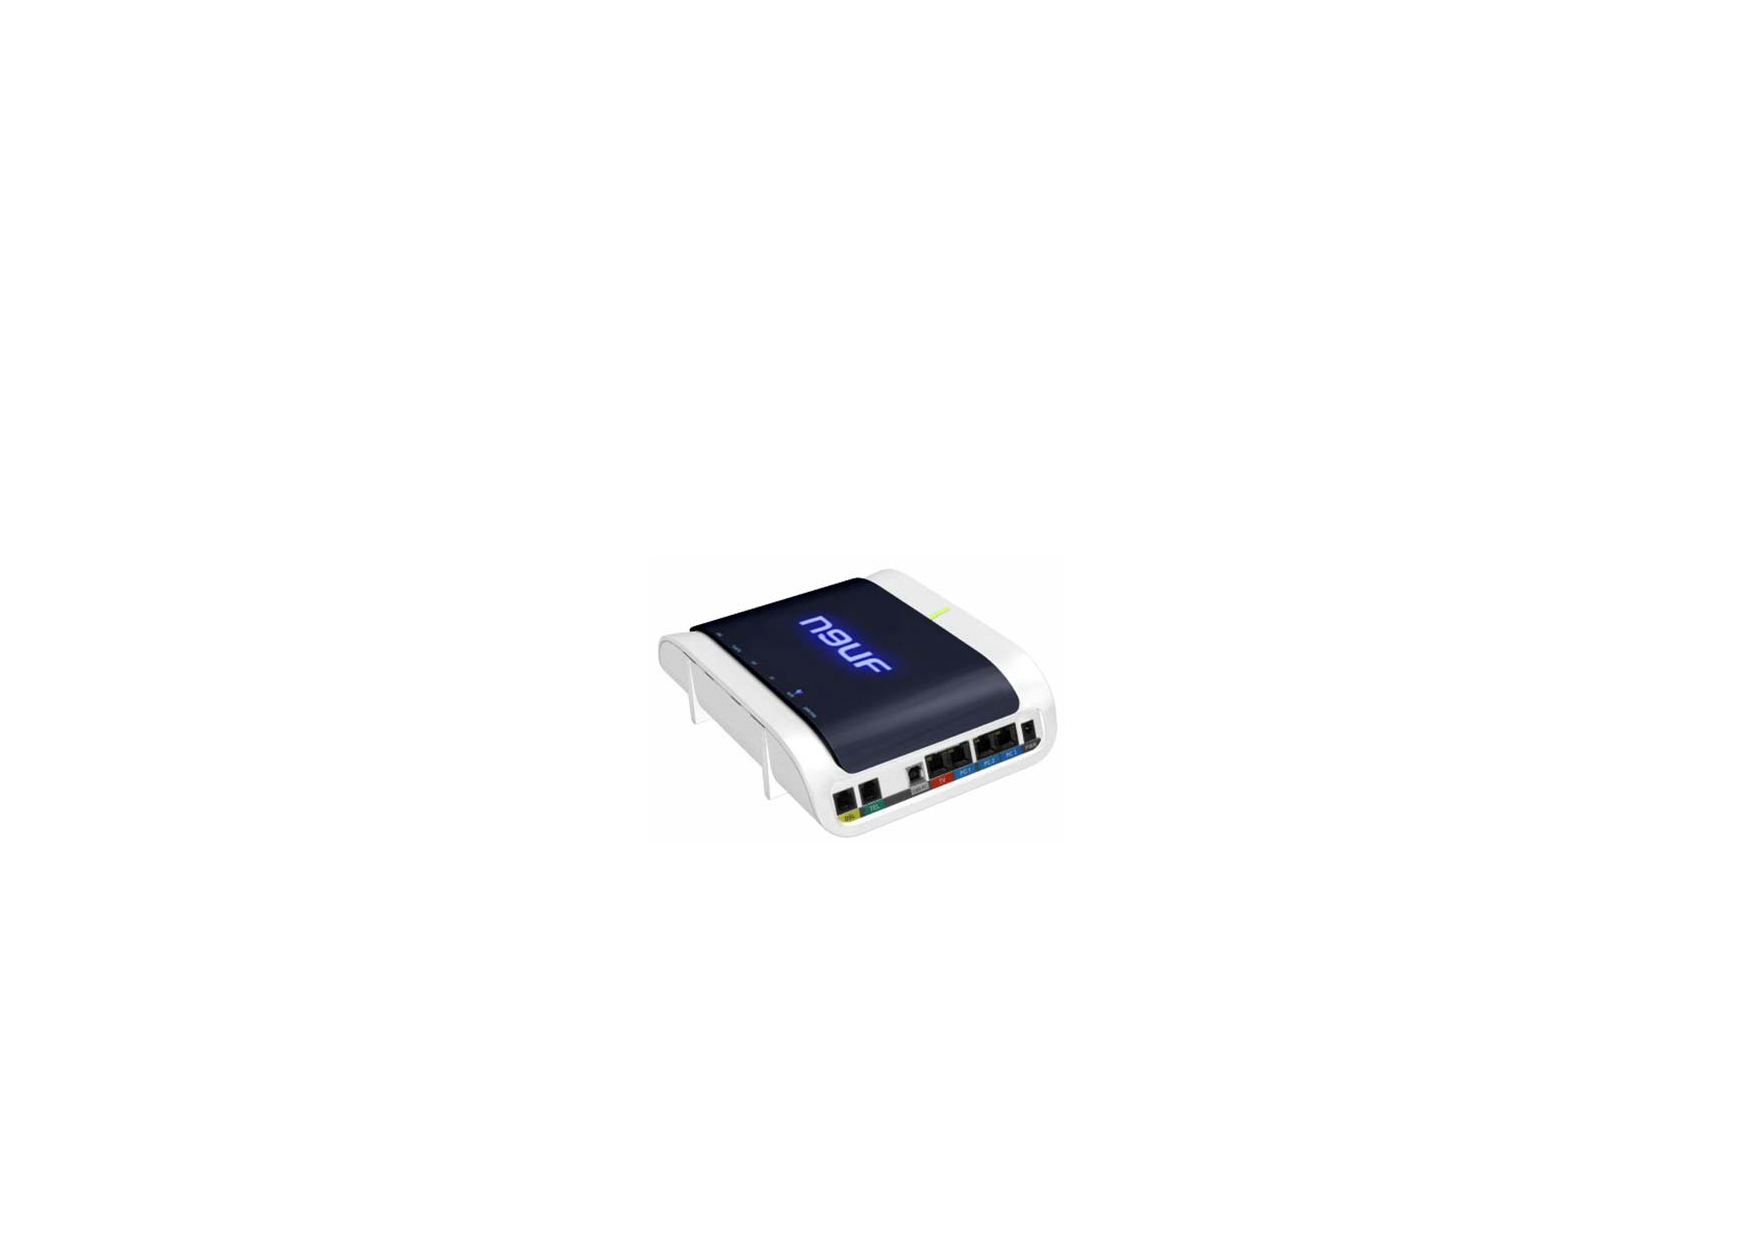
\includegraphics[width=\adslwidth]{\resdir/adslbox1.pdf}}\only<2>{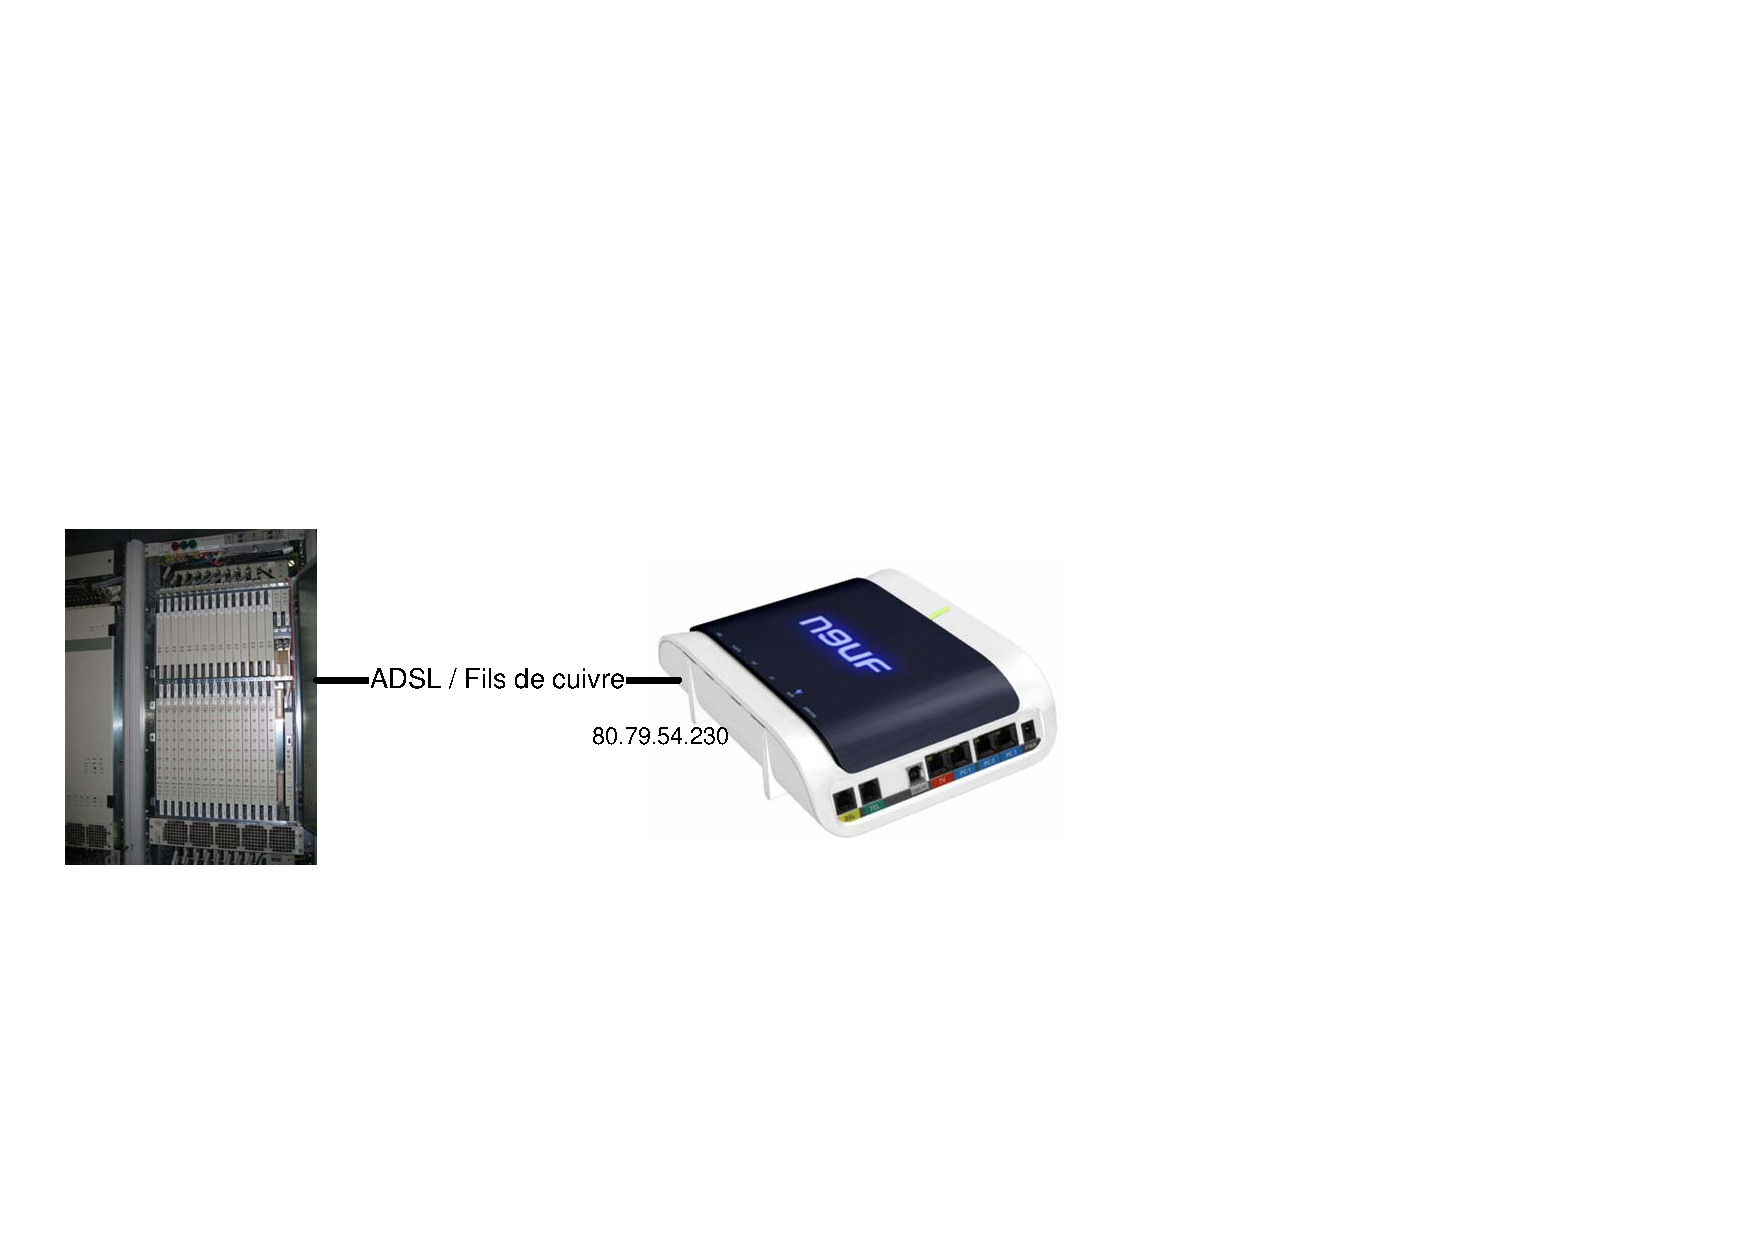
\includegraphics[width=\adslwidth]{\resdir/adslbox2.pdf}}\only<3>{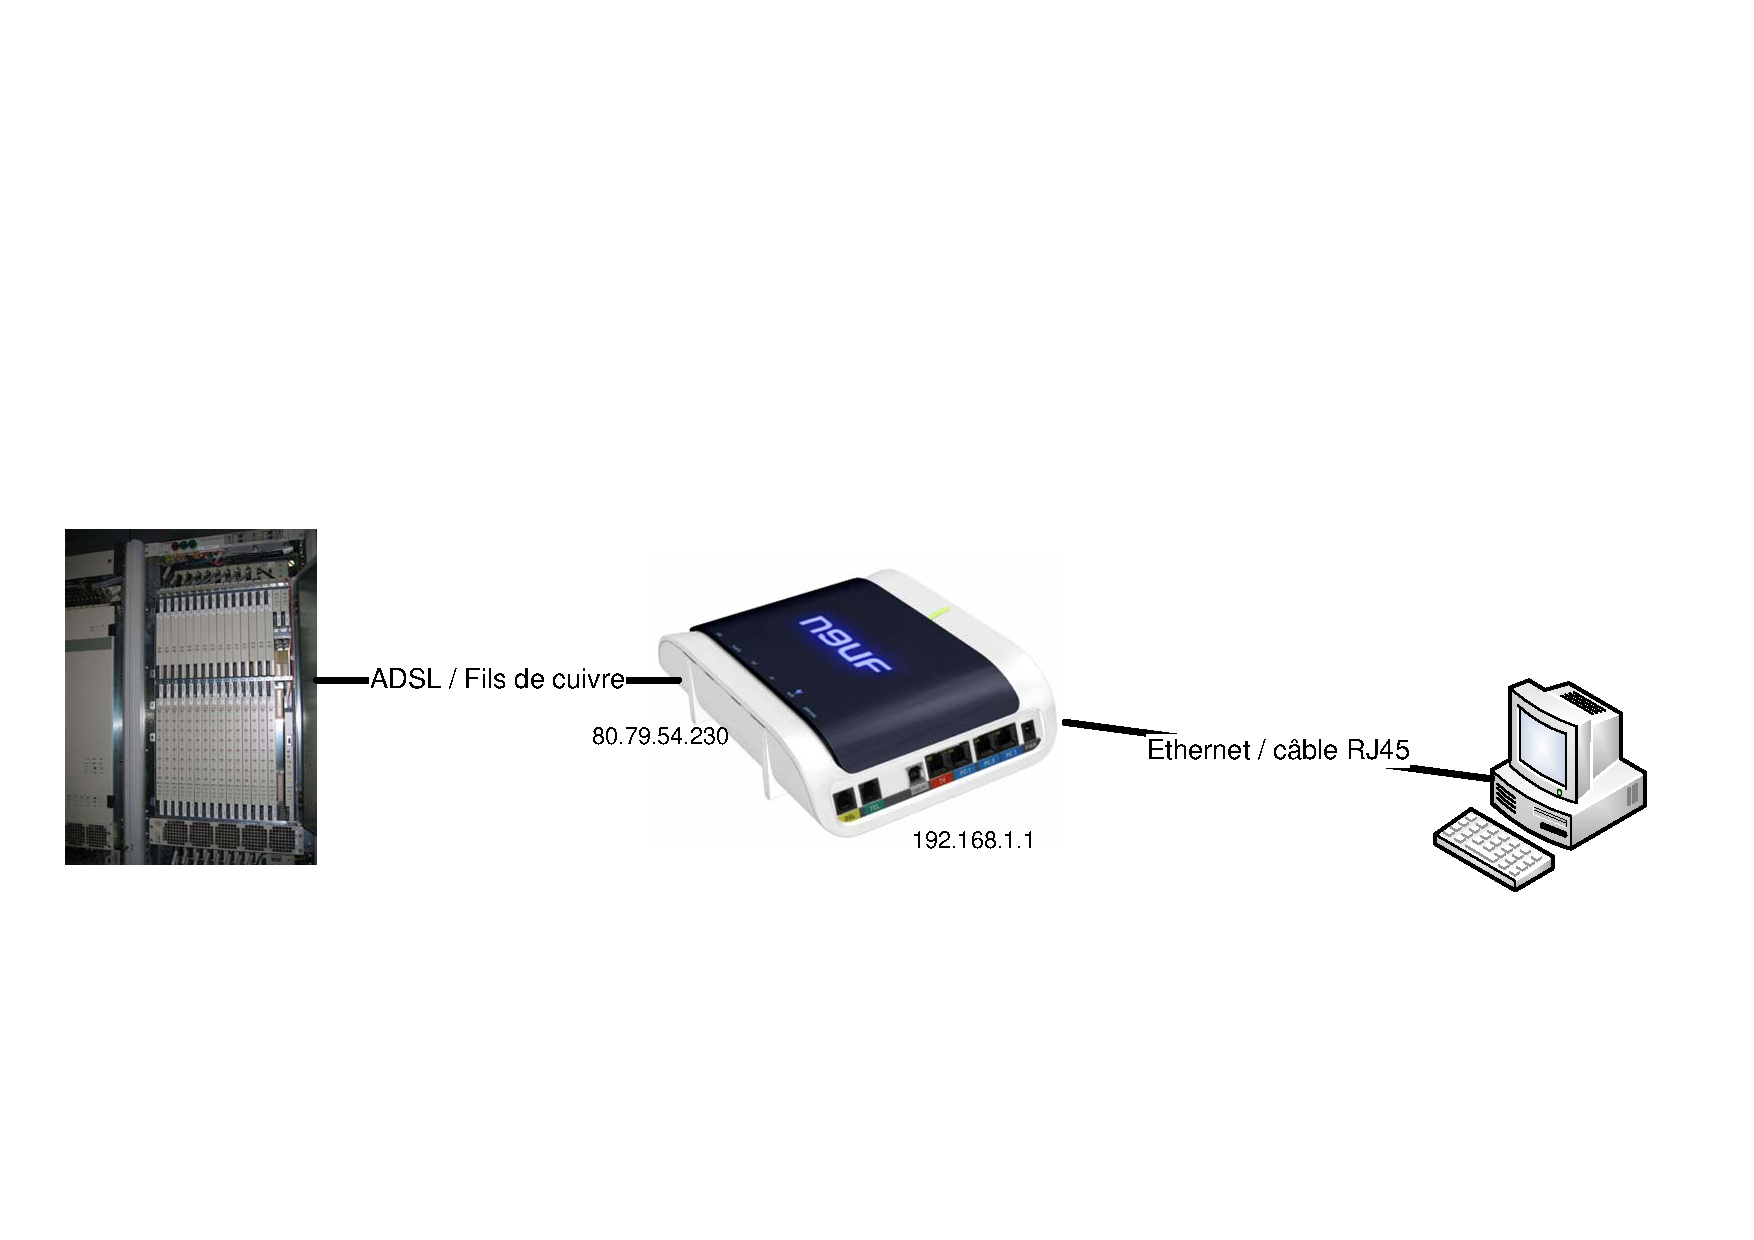
\includegraphics[width=\adslwidth]{\resdir/adslbox3.pdf}}\only<4>{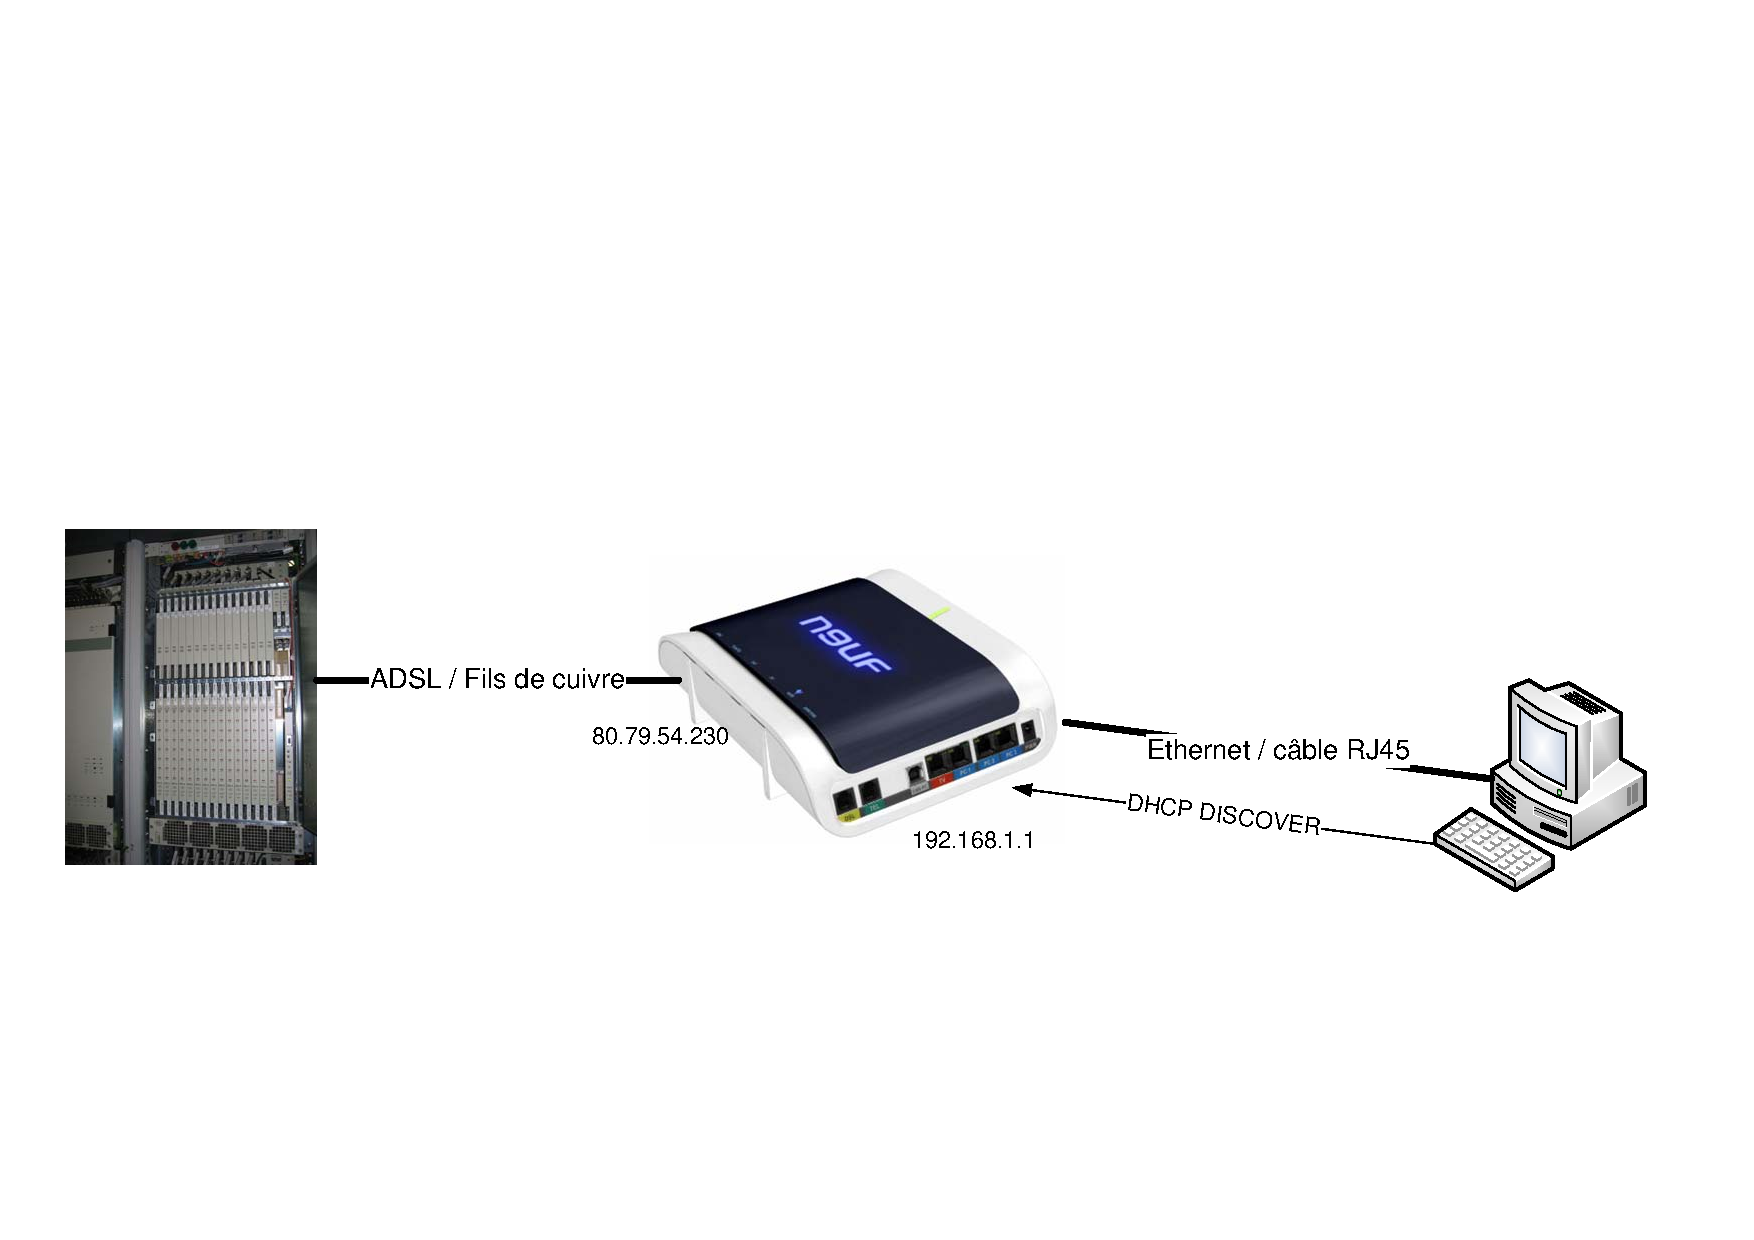
\includegraphics[width=\adslwidth]{\resdir/adslbox4.pdf}}\only<5>{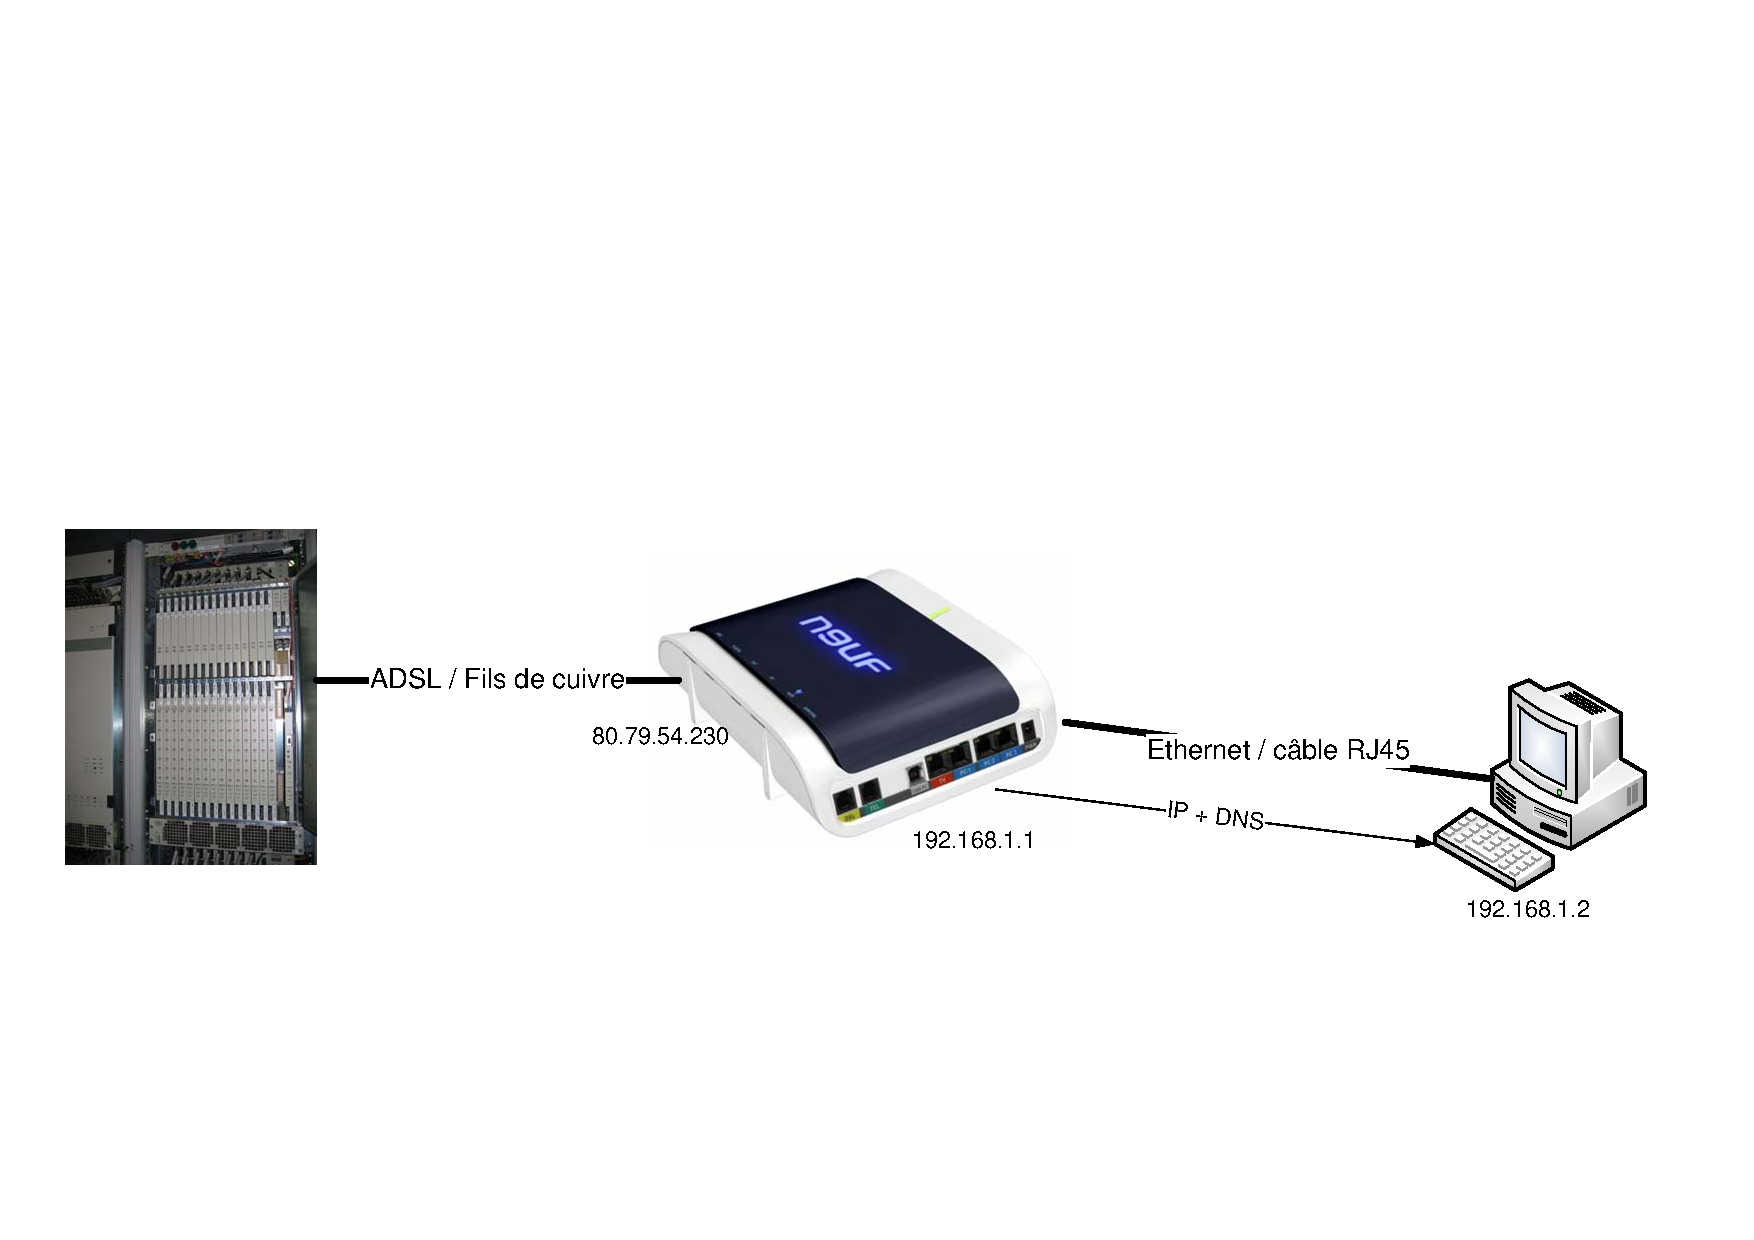
\includegraphics[width=\adslwidth]{\resdir/adslbox5.pdf}}\only<6>{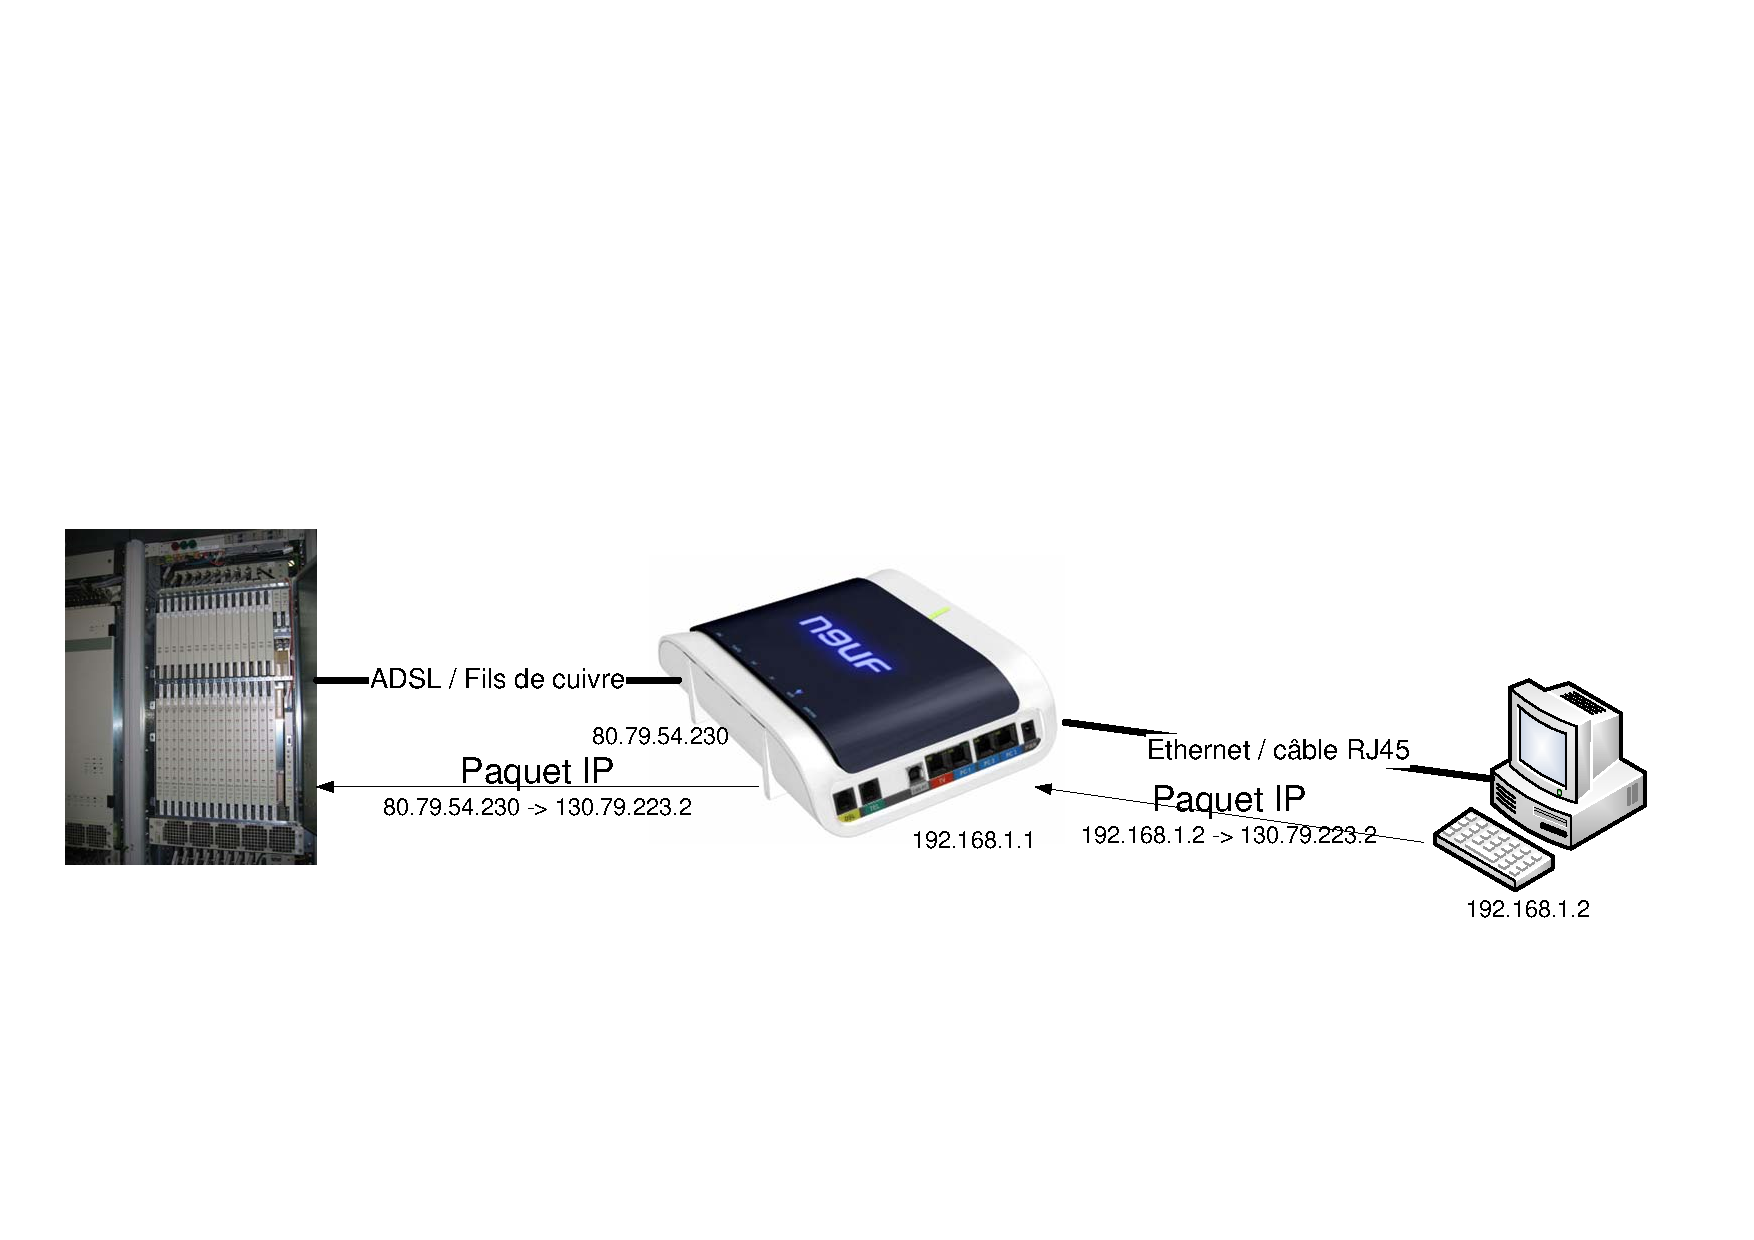
\includegraphics[width=\adslwidth]{\resdir/adslbox6.pdf}}\only<7>{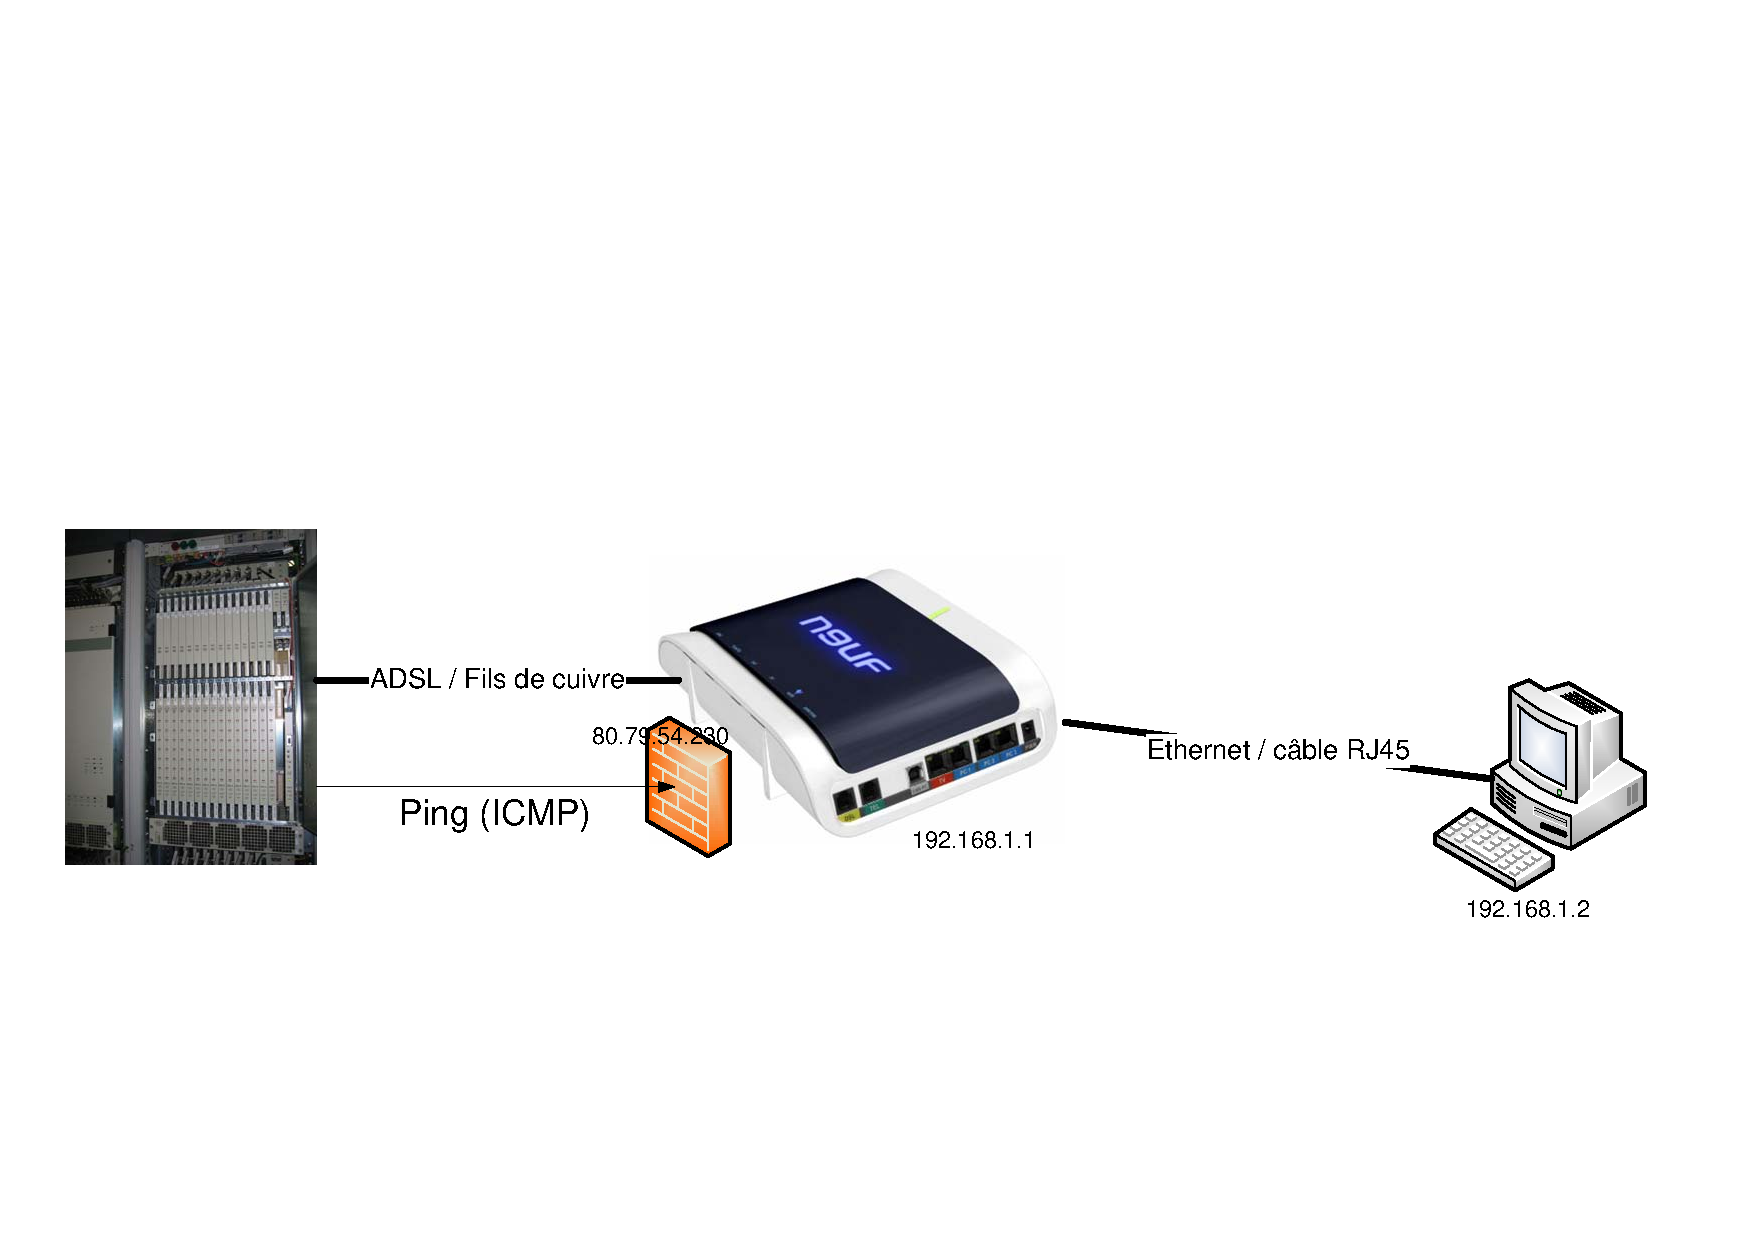
\includegraphics[width=\adslwidth]{\resdir/adslbox7.pdf}}\only<8>{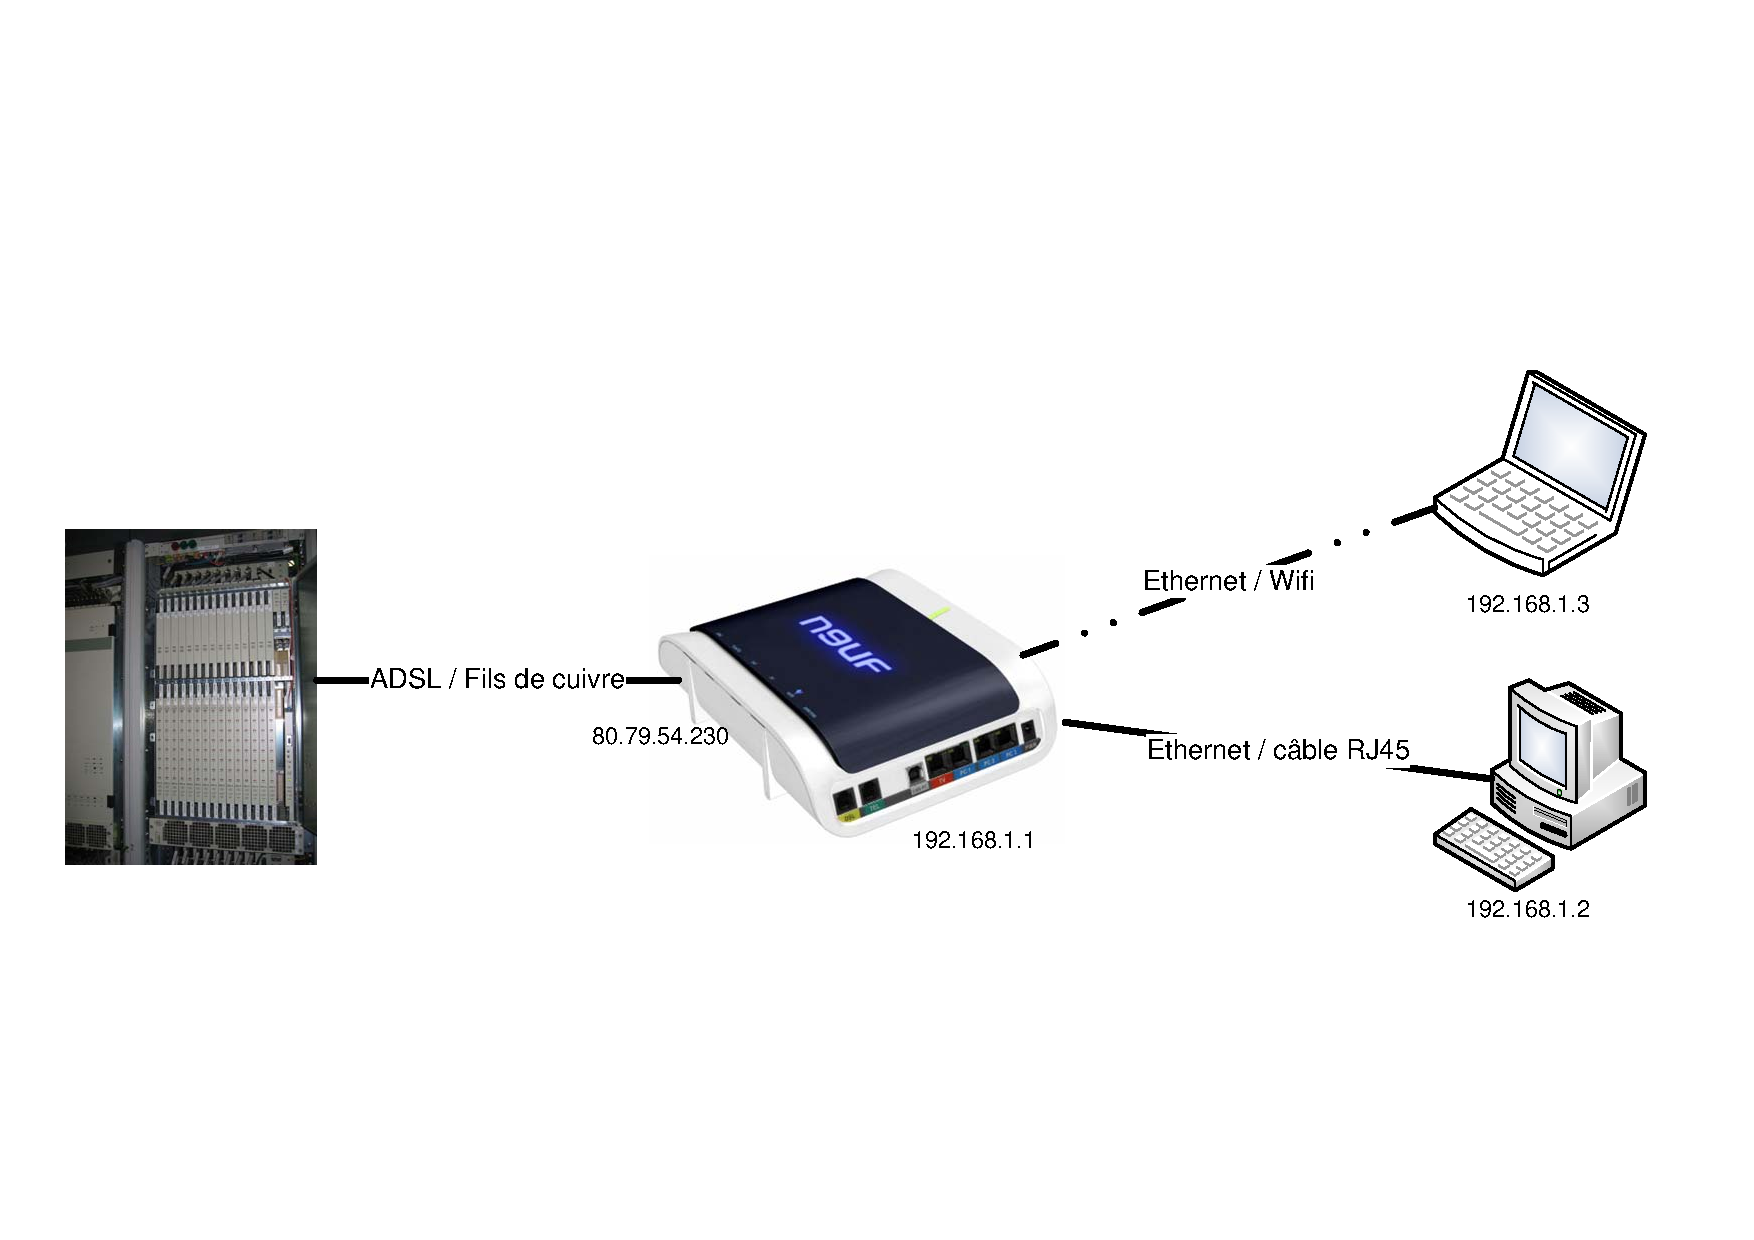
\includegraphics[width=\adslwidth]{\resdir/adslbox8.pdf}}\only<9>{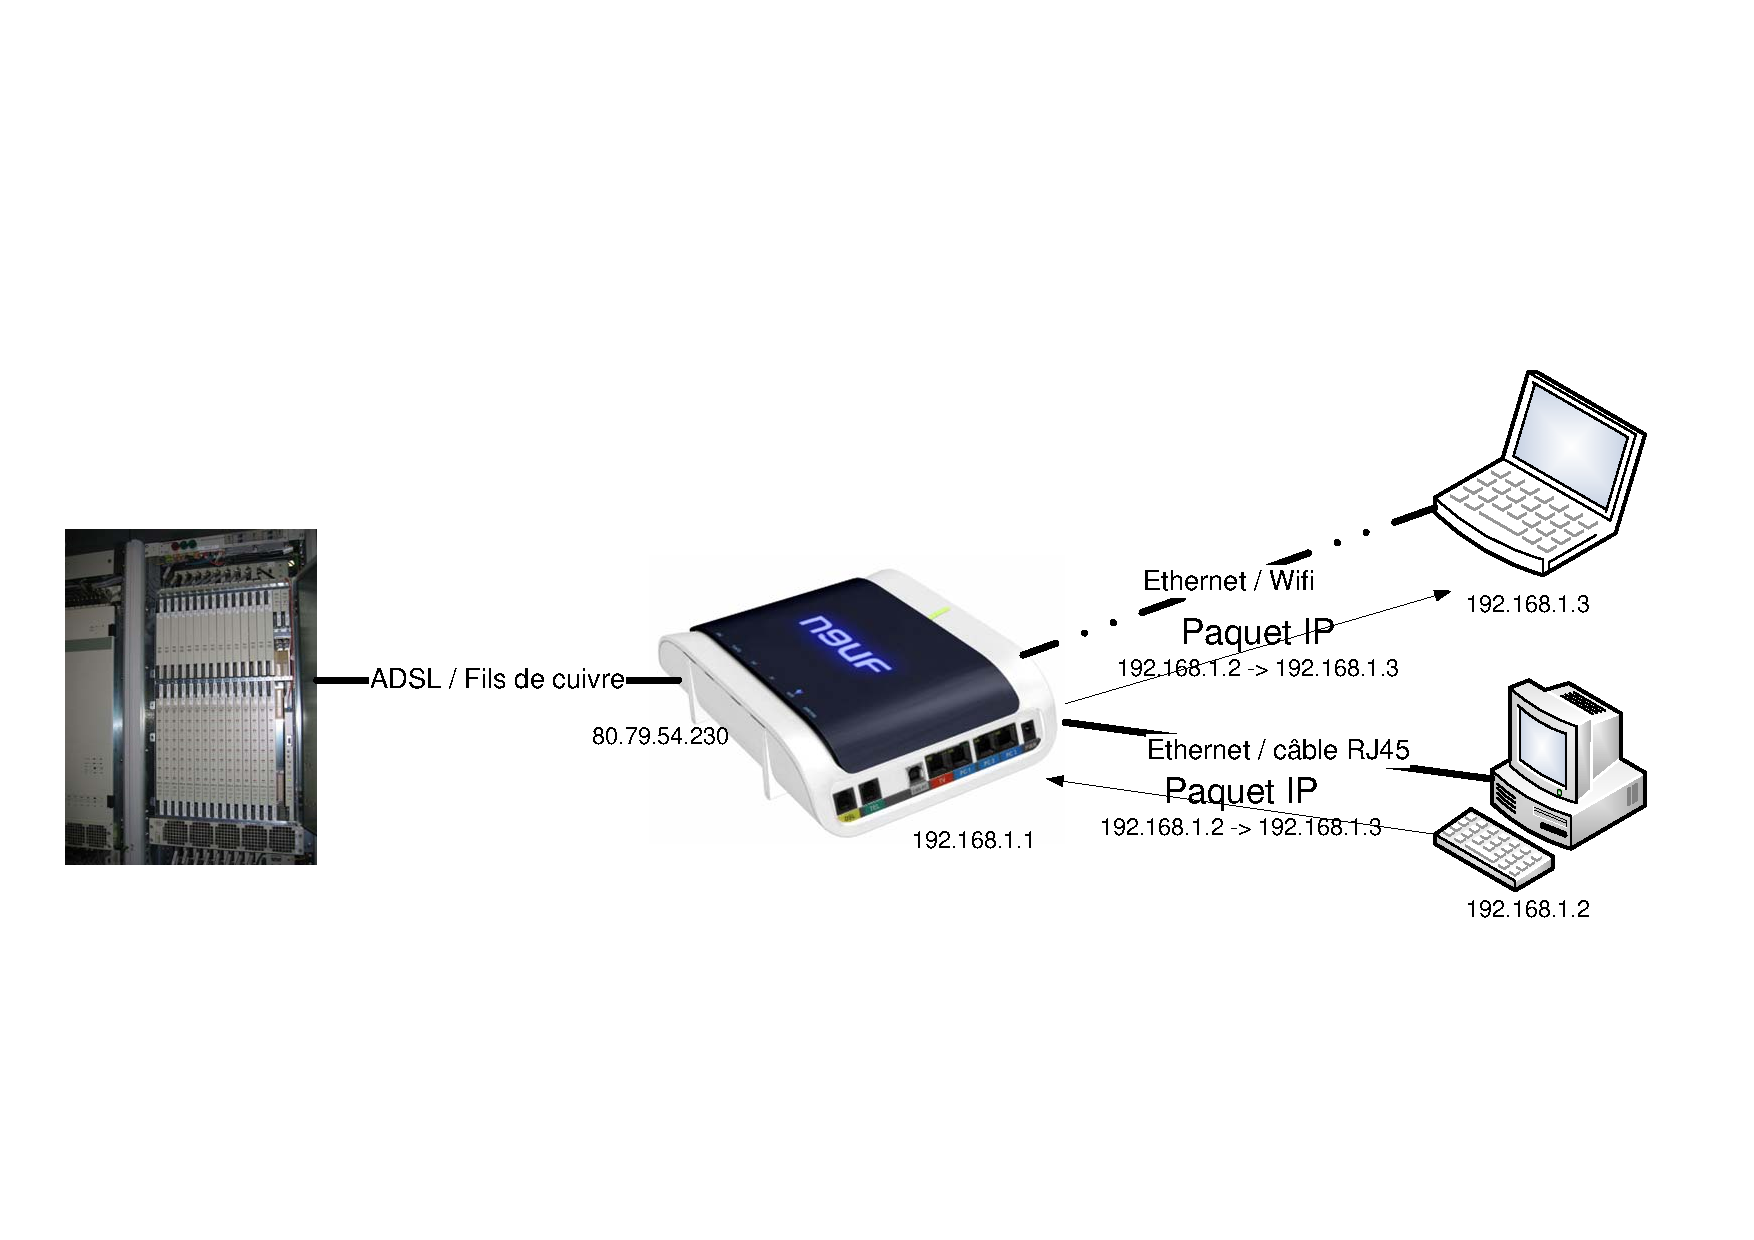
\includegraphics[width=\adslwidth]{\resdir/adslbox9.pdf}}\only<10>{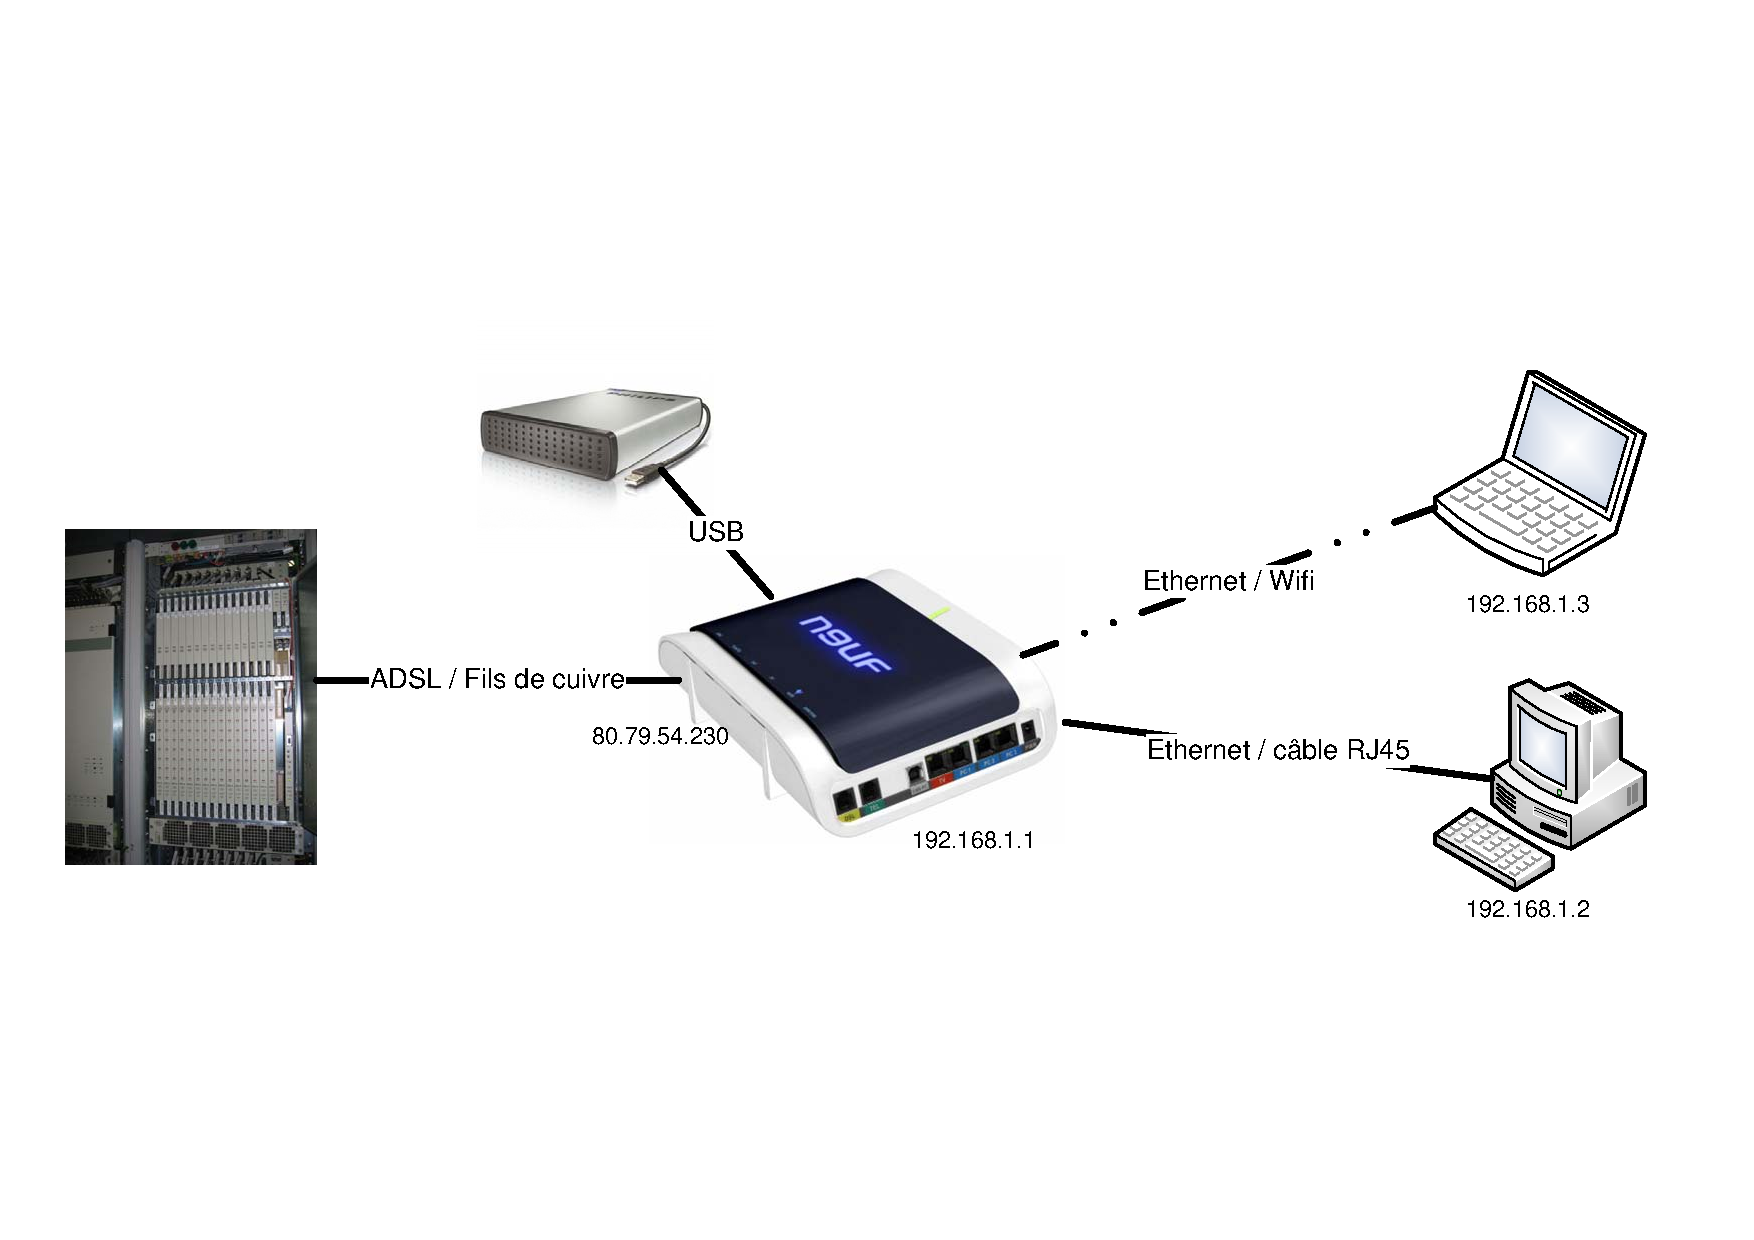
\includegraphics[width=\adslwidth]{\resdir/adslbox10.pdf}}\only<11>{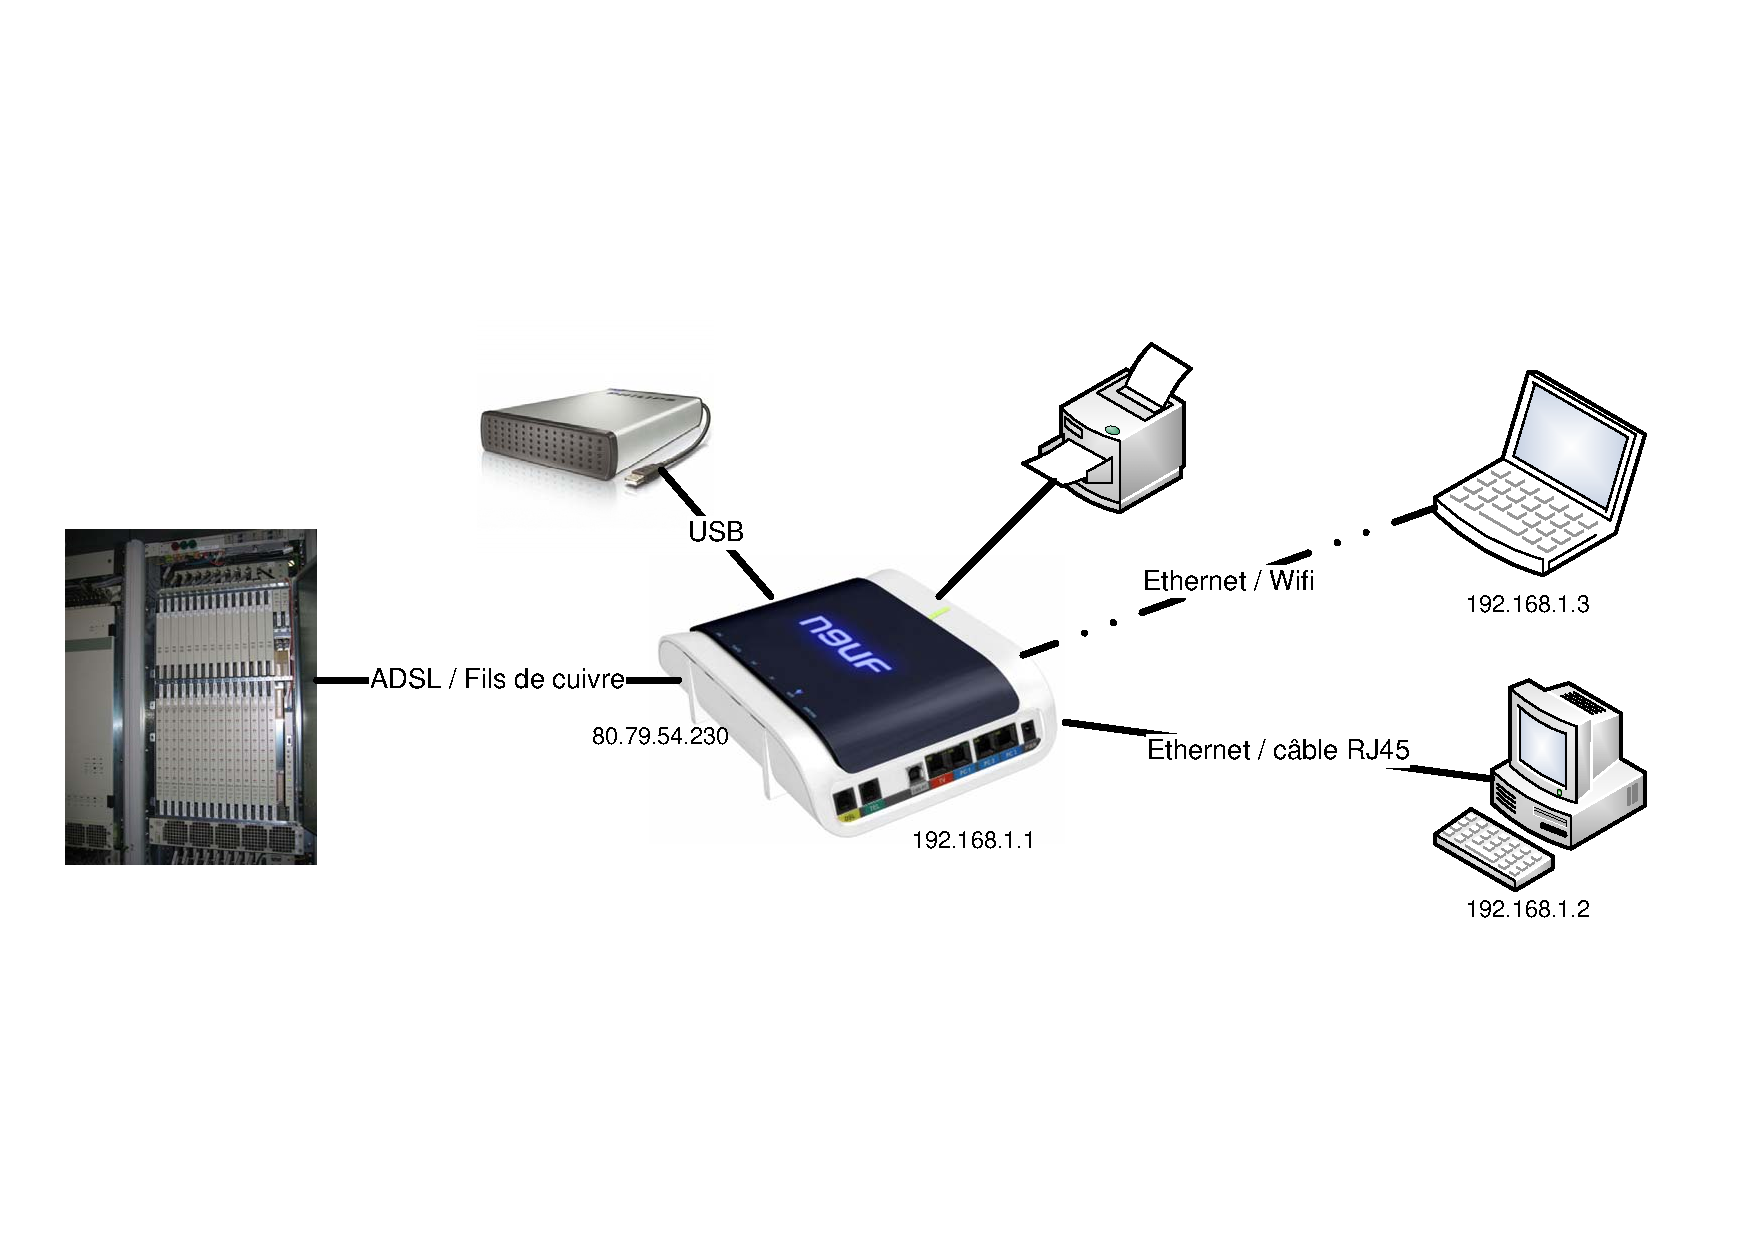
\includegraphics[width=\adslwidth]{\resdir/adslbox11.pdf}}

\vspace*{-2cm}

	\begin{block}<+-> {adslbox}
		\scriptsize
		\begin{columns}
			\begin{column}{0.35\textwidth}
				\begin{itemize}
				\item<3-> Pont
				\item<4-> Serveur DHCP
				\item<6-> Pont + Passerelle + Proxy
				\item<7-> Pare-feu
				\end{itemize}	
			\end{column}
			\begin{column}{0.65\textwidth}
				\begin{itemize}
				\item<8-> Hotspot Wifi (+ Serveur DHCP + WEP/WPA + Pare-feu)	
				\item<9-> Commutateur
				\item<10-> Serveur de fichier (FTP)
				\item<11-> Serveur d'impression
				\end{itemize}	
			\end{column}			
		\end{columns}
	\end{block}
	
\end{frame}
% ----------------------------------------------------------------------

